% For homework writeups, the Introduction section should state the general thrust of the assignment.

% What is the problem being studied? Explain in 2-3 sentences.

% What is the approach for studying the problem? Hint: the approach consists of the program(s) you are writing, so say in 2-3 sentences something about those programs. If you like, it is ok to use a forward reference, and say something like "we present the implementation in \S\ref{sec:implementation}. 

% What are the main results? Say something about the results in 2-3 sentences: what is the nature of your experiment that tests your implementation, and say something about the insights gained. 

% for each of the problem statement, approach statement, and findings/result statement from the abstract, amplify these into a short paragraph for each. Here, "short paragraph" means 3-4 sentences.

% State the objective for the implementation (2-3 sentences).

% The implementation of distributed-memory stencil operations aims to enhance computational performance by leveraging parallel execu- tion across multiple CPU nodes. Unlike shared-memory approaches, which are confined to a single node, distributed-memory imple- mentations partition workloads across nodes, each with its own memory space. 

This assignment explores the problem of implementing distributed-memory stencil operations using the Message Passing Interface (MPI)~\cite{mpi_spec} to enhance computational performance by leveraging parallel execution across multiple CPU nodes. Distributed-memory implementations partition workloads across nodes, each with its own memory space, enabling scalability for larger problems and efficient utilization of computational resources. The primary objective is to design and evaluate an efficient distributed Sobel filter for edge detection that achieves high performance and scalability through effective task partitioning and data communication strategies. Figure~\ref{fig:grayscale} presents the original grayscale image used for testing, while Figure~\ref{fig:sobel-output} shows the resulting image after applying the Sobel filter.

We divided the computational domain using three decomposition strategies: Row-slab, Column-slab, and Tiled. For efficient data exchange, we employed custom MPI datatypes, which were especially crucial when transferring non-contiguous memory regions. These datatypes optimized communication by reducing the number of messages between ranks. The Sobel filter operations were parallelized across nodes to exploit concurrency. Further details about the implementation are provided in Section~\ref{sec:implementation}.

The results of our experiments demonstrate that all decomposition strategies improve runtime performance of Sobel filtering with increasing concurrency, but the tiled decomposition strategy exhibits superior scalability thanks to its relatively even workload distribution. Additionally, the runtime for scattering and gathering was consistent across all decomposition methods and concurrency levels due to the use of subarray datatypes, which minimized and optimized inter-node communication. These findings highlight the critical role of balancing workloads and minimizing communication in optimizing distributed-memory stencil operations.

\begin{figure}[h]
    \centering
    \begin{subfigure}{0.45\textwidth}
        \centering
        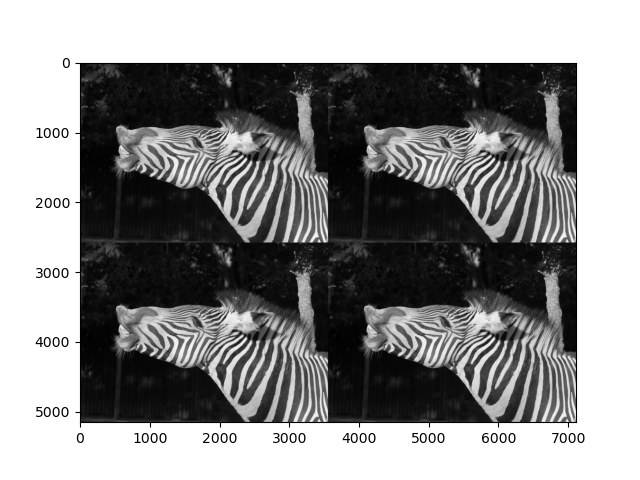
\includegraphics[width=\textwidth]{images/grayscale.png}
        \caption{Original Grayscale Image}
        \label{fig:grayscale}
    \end{subfigure}
    \hfill
    \begin{subfigure}{0.45\textwidth}
        \centering
        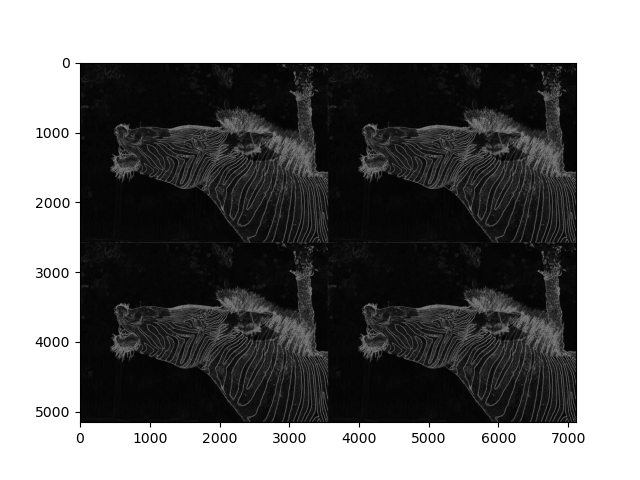
\includegraphics[width=\textwidth]{images/sobel_output.png}
        \caption{Sobel Filter Output}
        \label{fig:sobel-output}
    \end{subfigure}
    \caption{Example results showing the original grayscale image and the Sobel filter output.}
    \label{fig:example-results}
\end{figure}